\chapter{Experiments And Results}
\label{ch:results}

This chapter reports what the method of \autoref{ch:method} does when it is run. It has two parts, which follow the two levels of the pipeline. The first part, \autoref{sec:inner-loop-experiments}, isolates the inner loop. The outer loop is switched off and the bodies are given rather than selected. The question is what the evolved rules add to a base controller on a body that does not change: first to the generalist, on bodies it has never flown, then to a specialist, on the one body it was trained for. The second part, \autoref{sec:codesign-experiments}, runs the whole pipeline and compares it with the morphology-only control of \autoref{subsec:pipeline-control}. The comparison is made on the terms set by \autoref{ch:challenges}: whether an adaptation as cheap as this one changes which bodies the search finds.

Every experiment of the chapter uses the controllers, the plastic layer, the courses and the flights of \autoref{ch:method}, with the values of \autoref{tab:hebbian-parameters}, \autoref{tab:evaluation-courses} and \autoref{tab:pipeline-settings}. Where an experiment departs from them, the departure is stated with the result it belongs to. The base controllers are the generalist of \autoref{subsec:generalist-training}, trained once, and the specialists of \autoref{subsec:specialist-training}. Three specialists were trained for the reference drone with the same settings and different random seeds; unless a specialist is numbered, the first of them is meant. The evolutionary algorithms are taken from their reference implementations: CMA-ES from pycma 4.4.4 \cite{hansen2019pycma} and NSGA-II from DEAP 1.4.3 \cite{fortin2012deap}. The networks run in PyTorch 2.10 \cite{paszke2019pytorch} and the simulation in Genesis 0.3.7 \cite{genesis2024}. A run is identified by its random seed, which fixes the samples of CMA-ES, the forests and, where there is one, the first population of bodies. \autoref{tab:results-runs} lists the runs of the chapter.
% PROVENANCE: library versions from reproducibility/environment.txt of the runs (cma==4.4.4, deap==1.4.3, torch==2.10.0);
% Genesis 0.3.7 = the vendored genesis/ (chapter 4). Specialists: wp1_bix_single_65536_lstm_15_r0..r2; "the first" = r1
% (the one used in the generalist-vs-specialist run and in the first rules-on-specialist run), second = r0, third = r2.

\begin{table}[tb]
\centering
\small
% Local to this float: tighter rows and columns than the global settings of thesis.tex, and a top-aligned X column.
\renewcommand{\arraystretch}{1.25}
\setlength{\tabcolsep}{4pt}
\renewcommand\tabularxcolumn[1]{p{#1}}
\begin{tabularx}{\textwidth}{>{\raggedright\arraybackslash}p{1.25cm} >{\raggedright\arraybackslash}p{1.9cm} >{\raggedright\arraybackslash}p{2.2cm} >{\raggedright\arraybackslash}p{1.85cm} >{\raggedright\arraybackslash}X >{\raggedright\arraybackslash}p{1.95cm}}
\hline
Section & Base controller & Bodies & Flights per generation & Measured at every generation, on new forests & Runs, generations \\
\hline
\ref{subsec:results-generalist} & generalist & 64 drawn at random, moved every 4 generations & 245\,760 & the best rules and the frozen generalist on the reference drone, 4\,096 forests & 1, of 50 \\
\ref{subsec:results-generalist} & generalist & the reference drone & 12\,800 & the best rules, the frozen generalist and a frozen specialist, 2\,048 forests & 3, of 200 \\
\ref{subsec:results-specialist} & a specialist & the reference drone & 12\,800 & the best rules, the frozen specialist and the frozen generalist, 2\,048 forests & 3, of 200, one per specialist \\
\ref{sec:codesign-experiments} & generalist & 64, half replaced at every exam & 245\,760 & the exam every 4 generations (every 6 in two runs): the 8 best rules $\times$ 64 bodies $\times$ 480 forests of the exam course & 8, of 200 \\
\ref{sec:codesign-experiments} & generalist, rules held at zero & 64, half replaced at every exam & 245\,760, all in the exam & the exam every generation: the frozen generalist $\times$ 64 bodies $\times$ 3\,840 forests of the exam course & 8, of 88 \\
\hline
\end{tabularx}
\caption[Runs of this chapter]{Runs of this chapter. Every run uses 64 sets of rules per generation, the search course and the noise of \autoref{subsec:evaluation-flights}; a flight of the search is one set of rules, one body and one forest.}
\label{tab:results-runs}
\end{table}
% Rows checked 2026-09-25 against the finished local runs (src/WP2/experiments/thesis_inner_loop/): generalist seeds 5535 and 5536
% (plus, since 2026-10-02, the older run B of seed 5535, 2026-06-10_10-40-16: the third run of the second row),
% specialists r1/r0/r2 with seeds 5535/5536/5537, all 200 generations, all exit 0.
% Section 6.2 rows added 2026-09-29: 8 co-design runs (4 of 2026-08-10 incl. the two refresh-6 runs + 4 of batch_5) and 8 morphology-only runs.

\section{Inner Loop Experiments}
\label{sec:inner-loop-experiments}

The inner loop of \autoref{subsec:inner-loop} was designed to run inside the outer loop, on bodies that the outer loop keeps replacing. Run on its own, on bodies that are given once and for all, it answers a narrower question. This question is nevertheless the first one to ask: whether the rules add anything to a base controller, and what they add. On a fixed body nothing varies from one flight to the next but the forest, the commanded speed and the noise. The body, which \autoref{subsec:hebbian-why-output} presented as the quantity that varies between lifetimes and that fixed weights cannot anticipate, is the same in every flight. The fixed body is therefore the setting in which the argument for plasticity promises the least. It is also the setting in which whatever the rules do can be read most clearly: the frozen base controller flies the same body under the same conditions, so any difference between the two is the work of the rules.

Two experiments are reported. In the first the base is the generalist, which flies every body as a compromise (\autoref{subsec:generalist-training}). The rules are evolved on many bodies, as in the pipeline, and then on the reference drone alone. The specialist trained for that drone gives the scale of what the generalist leaves on the table there. In the second experiment the base is a specialist, a controller that was trained for the body it flies and has nothing to recover. There are three specialists, and the experiment is run on each of them.

\subsection{Recovering Performance on Generalist Controllers}
\label{subsec:results-generalist}

The first experiment runs the inner loop as the pipeline runs it, with one change: the bodies are not selected. Sixty-four bodies are drawn at random, as in the first generation of a run, with the reference drone excluded. Every four generations, each gene of each body is moved by a Gaussian step of standard deviation 0.02 in the unit cube. The population thus keeps changing under the rules, as it does in a run, but it drifts as a random walk instead of following the objectives. Fifty generations are run, with twelve such refreshes, and with the population, the flights and the fitness of \autoref{tab:pipeline-settings}: 64 sets of rules, 245\,760 flights of the search course per generation, forests drawn anew at every generation. At every generation the frozen generalist flies the same bodies on the same forests. In addition, the best set of rules of the generation and the frozen generalist fly the reference drone on 4\,096 further forests of the search course, which the search never sees; this is the measurement described in \autoref{subsec:pipeline-run}. The experiment thus shows the progress of the inner loop on the bodies it is given and on one body it is not given.
% PROVENANCE: logs/remote/wp2_evolution/wp2_mutation_4_bix_validation_lstm_15_r0/2026-06-13_02-23-30_mutation_4_bix_validation_lstm_15
% (IZAR, 27 h; catalog.mutate true, mutation_std 0.02, refresh_urdfs_every 4, include_standard_mydrone false, seed 67;
% production checkpoint, md5-identical to batch_5). Numbers: tesis/images/06_Results_and_Experiments/inner_loop/inner_loop_stats.json, "A".

\begin{figure}[htbp]
\centering
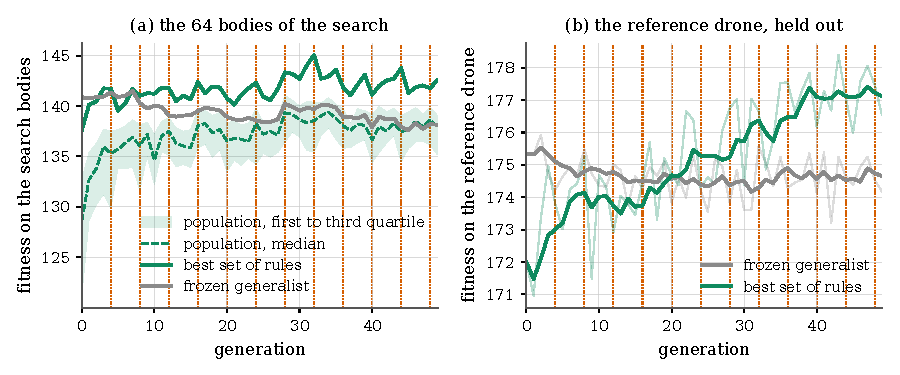
\includegraphics[width=\textwidth]{images/06_Results_and_Experiments/inner_loop/inner_loop_bodies.pdf}
\caption[The inner loop on 64 random bodies]{The inner loop on 64 random bodies. (a) Fitness on the bodies of the search: the best of the 64 sets of rules of each generation, the population's median with a band from the first to the third quartile, and the frozen generalist on the same bodies and forests. The dotted lines mark the refreshes of the bodies. (b) The best set of rules of each generation and the frozen generalist on the reference drone, which the search never flies, over 4\,096 new forests per generation; thin lines are the raw values, thick lines a moving average over five generations.}
\label{fig:inner-loop-bodies}
\end{figure}

\autoref{fig:inner-loop-bodies}(a) shows the fitness on the bodies of the search. At the first generation every one of the 64 sets of rules flies worse than the frozen generalist: the population's median is 129 against 141 for the frozen controller, and its best is 138. This is the starting point that \autoref{subsec:inner-loop} chose. The rules begin as small perturbations of a controller that flies, and a perturbation, on average, costs. From there CMA-ES moves. From the seventh generation on, the best set of rules of each generation is above the frozen controller. Over the last ten generations the best set exceeds the frozen controller by 3.9, 142.2 against 138.2, a gain of about 3\,\%; the step size has shrunk from 0.074 to 0.058 in the meantime. The population's median, however, only catches up with the frozen controller, 137.9 against 138.2 over the same generations, and its upper quartile barely passes it. The search has found a direction in which the rules help, but a random perturbation around that direction still costs about as much as the direction gains. The population as a whole never becomes clearly better than the controller without rules. The curve of the frozen controller is not flat, because at every refresh the bodies change and the new population flies a little differently. This is the reason given in \autoref{subsec:pipeline-run} why the fitness of the rules cannot be compared across updates of the bodies. The comparison that the figure allows is the one that holds at every generation: between the rules and the frozen controller, on the same bodies and forests.

Panel (b) is the same comparison on a body that the search never flies. On the reference drone the best rules of the first generation are worse than the frozen generalist by 3.4, and they remain worse for the first four phases, sixteen generations: rules selected on other bodies do not transfer at once. From the sixth phase on the sign is reversed. Over the last ten generations the best rules exceed the frozen controller by $2.5 \pm 0.6$ on the reference drone, 177.1 against 174.6, or 1.4\,\%. The uncertainty is the spread over generations of the paired difference, each measured on 4\,096 fresh forests. The fitness of the frozen controller alone varies by 0.6 from one generation's forests to the next, so the gain is well above what a draw of forests can produce. The gain is also two thirds of what the rules gain on the bodies they are evolved on. This is the expected direction: part of what a set of rules gains is specific to the bodies on which it was selected.

Decomposed into the quantities of the flights, the held-out gain is of one kind. Progress and the fraction of flights that end in a crash, in the sense of \autoref{subsec:reward}, barely move: 117.2~m against 116.8~m, and 52\,\% of the flights lost against 53\,\%, on a course that ends at five trees per metre. What moves is the speed and the energy. The rules lower the speed by 2\,\%, from 13.9 to 13.6~m/s over commands between 10 and 20~m/s, and they lower the energy per metre more, by 4\,\%. The rules do not make the generalist a better pilot of the reference drone in the sense in which a specialist is one. They make it fly the same course, with the same losses, a little slower and cheaper, and the reward pays for the change. Its energy term rewards the saving directly. Its tracking term is a bell curve that is flat near the commanded speed, so a flight a few per cent slower costs almost nothing per step, while the flight lasts longer over the same distance. The first generations show the opposite, a cost of transport above that of the frozen controller, and the search passes through it. Which term of the reward the rules end up serving is not decided at the start.

How much of what the generalist loses on the reference drone is this? The specialist trained for that drone gives the measure. In a second run the rules were evolved on the reference drone alone, with the same population and 200 forests for each set of rules, 12\,800 flights per generation, for 200 generations. At every generation the best set of rules, the frozen generalist and the frozen specialist flew 2\,048 fresh forests of the search course. \autoref{fig:inner-loop-reference-generalist} shows the three curves. The frozen generalist scores 174.5 on the reference drone and the specialist 182.2. The gap of 7.7, or 4\,\%, is the price of the compromise of \autoref{sec:challenge-morphology} on a body of ordinary proportions. The rules, evolved on this body alone, recover $3.4 \pm 1.2$ of the gap over the last fifty generations, that is 44\,\% of it. The gain appears within the first twenty generations, reaches 3 by the sixtieth and hardly moves afterwards. The gap itself depends on which specialist is used as the measure. The three specialists that were trained score 182.2, 189.7 and 182.4 on the same kind of forests (\autoref{subsec:results-specialist}), so the rules recover between a quarter and a half of what a specialist has over the generalist.
% PROVENANCE: logs/runs_hebbian/2026-09-24_20-15-15_rules_on_generalist_s5535 (local, 200 gens, seed 5535, specialist r1;
% 22:15 → 03:17 on 2026-09-25, exit 0). Window = generations 150 to 199. inner_loop_stats.json, "G"[first entry].

\begin{figure}[htbp]
\centering
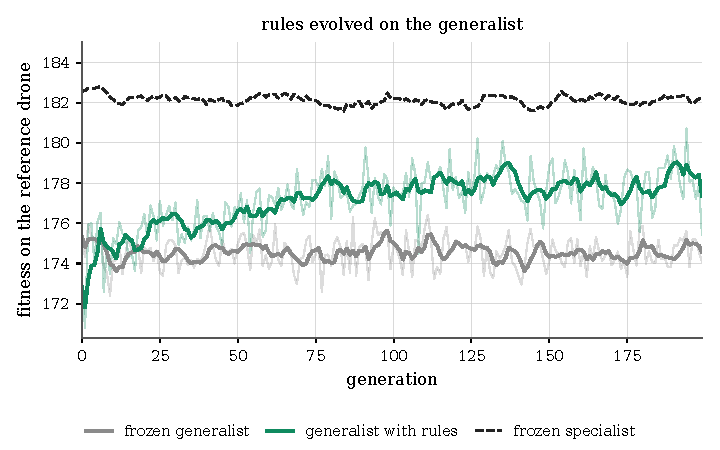
\includegraphics[width=0.8\textwidth]{images/06_Results_and_Experiments/inner_loop/inner_loop_reference_generalist.pdf}
\caption[The inner loop on the reference drone alone, generalist base]{The inner loop on the reference drone alone, with the generalist as base: fitness of the best set of rules of each generation, of the frozen generalist and of the frozen specialist, over 2\,048 new forests per generation flown by all three. Thin lines are the raw values, thick lines a moving average over five generations.}
\label{fig:inner-loop-reference-generalist}
\end{figure}

But the two gains are of a different kind. The specialist loses 28\,\% of its flights where the generalist loses 53\,\%, and it covers 124~m where the generalist covers 117~m. It flies at the same speed as the generalist to within a tenth of a metre per second, and it spends more per metre, with a cost of transport of 0.32 against 0.28. The rules leave the losses and the progress where the generalist has them, and they lower the cost of transport by 9\,\%, to 0.26, at a speed 3\,\% lower. Measured in reward, the rules recover over two fifths of the gap. Measured in what the body does, they recover none of the specialist's advantage, which lies in avoiding the trees, and they find instead an economy that the specialist never looked for. In the terms of the objectives of \autoref{subsec:outer-loop} the two changes are not on the same axis. The specialist moves the body along progress and pays for it in energy; the rules move it along the cost of transport at constant progress. This is the approximate correspondence between the reward and the objectives of which \autoref{subsec:reward} warned, seen from the side of the search: a change that the reward pays for need not be the change that a specialist would have made.

Two further observations from this run are used later. The first concerns the selection. The fitness with which the best set of rules is selected, on the forests of the search, is 182.0 over the last fifty generations, against 177.9 for the same set of rules on the held-out forests. The maximum of 64 noisy measurements is thus optimistic by about 4, and a set of rules that is the best of its generation by that margin has often only been lucky on that generation's forests. This is one of the reasons why the pipeline evaluates the bodies on new forests and under eight sets of rules rather than one (\autoref{subsec:outer-loop}). The second concerns repeatability. The run was repeated once with the same seed and once with another seed, for 200 generations each. Runs with the same seed diverge in the simulator, as every run does (\autoref{subsec:genesis-proscons}). The two repeats nevertheless agree with the first run in the result, with gains of 4.5 and $3.6 \pm 1.0$ over their last quarters and the same decomposition into speed and energy.
% PROVENANCE: winner's curse = search_best_last - val_best_last of the 200-gen run; repeats = run B (below) and the second seed.
% Run C, logs/runs_hebbian/2026-07-08_09-59-42_validation_wspecialis_15_no_bix_15_lstm (100 gens, gain gens 75-99 +3.0), was
% dropped from the text on 2026-10-02 (author's decision, B5 of reviews/2026-10-01_review.md). Run B:
% logs/runs_hebbian/2026-06-10_10-40-16_validation_wspecialist_no_bix_15_lstm (200 gens, gain gens 150-199 +4.5; its
% "specialist" line is a 25-step specialist and is not used) and the second seed logs/runs_hebbian/2026-09-25_09-11-59_rules_on_generalist_s5536
% (200 gens, seed 5536, specialist r0 as third line: gain gens 150-199 +3.57 ± 0.97, CoT 0.261/0.285, speed 13.33/13.89).

\subsection{Improving Performance on Specialist Controllers}
\label{subsec:results-specialist}

The second experiment repeats the last one with a specialist in the place of the generalist, once for each of the three specialists trained for the reference drone. The rules are evolved on top of the frozen specialist, on the reference drone, with the same population, the same 12\,800 flights per generation and 200 generations. At every generation the best set of rules, the frozen specialist and the frozen generalist fly 2\,048 fresh forests. Whether the rules can help a specialist was left open in \autoref{subsec:specialist-training}. A specialist was trained for the body it flies. The argument of \autoref{subsec:hebbian-why-output}, that plasticity is selected when something varies between lifetimes, gives the rules nothing to work on here, because the body is the one the weights were trained for. The question is whether a controller that already fits its body leaves the rules anything to improve, and, if it does, what.
% PROVENANCE: logs/runs_hebbian/2026-09-24_16-47-43_rules_on_specialist_r1_s5535 (first specialist), 2026-09-25_01-17-04_rules_on_specialist_r0_s5536
% (second), 2026-09-25_05-45-56_rules_on_specialist_r2_s5537 (third); local, seeds 5535/5536/5537, all exit 0; the "specialist_*" columns of their
% validation_summary.csv hold the frozen generalist. Window = generations 150 to 199. inner_loop_stats.json, "S". Generalist row of the table = run 2.

\begin{table}[htbp]
\centering
\small
\begin{tabularx}{\textwidth}{>{\raggedright\arraybackslash}X r r r r r r r r r}
\hline
 & \multicolumn{4}{c}{frozen} & \multicolumn{5}{c}{with the best rules} \\
Base controller & fitness & speed & CoT & crashes & fitness & gain & speed & CoT & crashes \\
\hline
generalist & 174.5 & 13.9 & 0.285 & 53\,\% & 177.9 & +3.4 & 13.4 & 0.259 & 53\,\% \\
first specialist & 182.2 & 13.9 & 0.320 & 28\,\% & 191.9 & +9.6 & 13.3 & 0.257 & 28\,\% \\
second specialist & 189.7 & 13.3 & 0.215 & 31\,\% & 190.2 & +0.5 & 13.3 & 0.212 & 34\,\% \\
third specialist & 182.4 & 13.9 & 0.344 & 29\,\% & 192.3 & +9.9 & 13.3 & 0.243 & 28\,\% \\
\hline
\end{tabularx}
\caption[The four base controllers on the reference drone, frozen and with the best rules]{The four base controllers on the reference drone, frozen and with the best set of rules of each generation, over the last fifty generations of their runs: fitness, mean speed along the corridor in m/s, cost of transport and fraction of flights ended by a crash, on 2\,048 new forests per generation. The gain is the difference in fitness between the two, measured on the same forests; its spread over generations is 1.2, 1.2, 1.0 and 0.8 from top to bottom.}
\label{tab:inner-loop-bases}
\end{table}

\begin{figure}[htbp]
\centering
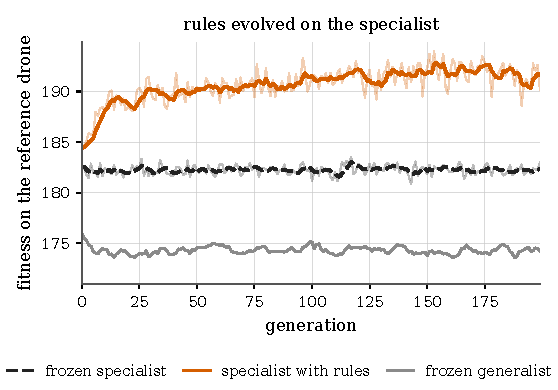
\includegraphics[width=0.62\textwidth]{images/06_Results_and_Experiments/inner_loop/inner_loop_reference_specialist.pdf}
\caption[The inner loop on the reference drone alone, specialist base]{The inner loop on the reference drone alone, with the first specialist as base: fitness of the best set of rules of each generation, of that specialist frozen and of the frozen generalist, over 2\,048 new forests per generation flown by all three. Thin lines are the raw values, thick lines a moving average over five generations.}
\label{fig:inner-loop-reference-specialist}
\end{figure}

\autoref{tab:inner-loop-bases} gives the answer, and it is not the same for the three specialists. On the first and the third specialist the rules add more than anywhere else in this section: $9.6 \pm 1.2$ and $9.9 \pm 0.8$, over 5\,\%, three times what they added to the generalist. \autoref{fig:inner-loop-reference-specialist} shows the first specialist. The rules are above the frozen specialist from the first generation, by 1.8 at generation 0 and by 4.3 over the first ten generations. The gain reaches 7.8 by the fortieth generation and 9.0 by the hundredth, and the third specialist follows the same course. On the second specialist the rules add nothing: $0.5 \pm 1.0$, negative over the first ten generations and inside the noise ever after.

The frozen controllers explain the difference. The three specialists were trained with the same settings and differ in the random seed alone, and they did not arrive at the same way of flying the reference drone. The first and the third fly it at 13.9~m/s with a cost of transport of 0.32 and 0.34, dearer than the generalist. The second flies it at 13.3~m/s with a cost of transport of 0.215, and it scores 7.5 more than the other two for it, with the same progress and the same crashes. The rules bring the first and the third specialist down to 13.3~m/s and to a cost of transport of 0.26 and 0.24, with progress and crashes untouched, as they brought the generalist from 13.9 to 13.4~m/s and from 0.285 to 0.259. The second specialist is there already, and the rules leave it where it is. Two further differences from the generalist's run are worth noting on the first specialist. The gain is there from the start, in the first generation, which is drawn with the same seed in the two runs; on the generalist, the best of the first generation was worse than the controller without rules. And the selection is less deceived by its own forests: the best fitness on the search forests exceeds the held-out fitness of the same rules by 2.5 instead of 4. The flights of a specialist vary less from one forest to the next, as its fewer crashes suggest.

Where the four bases end up is the remarkable part, and \autoref{tab:inner-loop-bases} shows it. Under their respective rules, the generalist and the three specialists all fly the reference drone at the same speed, 13.3 to 13.4~m/s, three of them down from 13.9~m/s. The cost of transport ends between 0.21 and 0.26. It is lowest for the specialist that was already there and highest for the generalist. Progress and crashes stay where each frozen controller had them. The rules do not move each controller by a fixed amount. They move each controller towards a slower and cheaper flight of the same course, the flight that the fitness of \autoref{subsec:inner-loop} rewards on this body. What each controller gains is the distance it had to travel to get there: nothing for the specialist that was there already, 3.4 for the generalist, about ten for the two specialists that flew fastest and dearest. Why the training reached this point with one seed and not with the other two, the experiment does not say. The training optimizes the discounted return of \eqref{eq:generalist-objective} from randomized releases, and the search optimizes the reward summed over a flight from a fixed release; the two are not the same measure of a flight.

This is how the gains of this section are to be read. \emph{Where a base controller ends up under the rules does not depend on where it started.} The speed at which the rules settle, and the slower and cheaper flight that goes with it, are a property of the body and of the fitness rather than of the controller, and a controller gains what it had to travel to get there. On a fixed body, then, the rules do what \autoref{sec:hebbian-controller} asked of them. They take a controller trained for all bodies, or a controller trained for this body but to a different flight, and they fit it to the flight of this body that the fitness rewards. They do so within a few tens of generations, on any base that is not there already. The gain is real in the currency of the outer loop, because a lower cost of transport at equal progress is a better point in objective space. What a fixed body cannot show is the case that \autoref{subsec:hebbian-why-output} made for plasticity: a body that differs from one flight to the next, which the controller must fit without being told which one it is. That is what \autoref{sec:codesign-experiments} is for.

\section{Full Co-Design Experiments}
\label{sec:codesign-experiments}

The second part of the chapter runs the pipeline of \autoref{sec:pipeline} as a whole and compares it with the control of \autoref{subsec:pipeline-control}. Eight co-design runs and eight morphology-only runs were made with the settings of \autoref{tab:pipeline-settings}, on eight random seeds. Six of the seeds carry a run of each condition, and the two runs of a seed start from the same 64 random bodies. The other two seeds carry a morphology-only run only. Two of the six shared seeds carry a second co-design run in which a phase lasts six generations instead of four, so that the run holds 33 phases instead of 50. All sixteen runs enter every comparison that treats the runs as independent. The paired analysis of \autoref{subsec:results-pca} uses the six shared seeds, with one co-design run for each. The morphology-only runs, whose bodies are updated at every generation, have 88 generations, 87 exams and 5\,568 examined bodies, against 49 exams and 3\,136 bodies for a co-design run. They took about 130 hours of the node against 94.
% PROVENANCE: co-design = logs/remote/outer_nsga/outer_exam_4_64_64_300_{r0,r1} (seeds 67, 68), outer_exam_6_64_64_300_{r0,r1}
% (seeds 67, 68, refresh 6), outer_exam_4_64_64_300_extra_r{0..3} (seeds 12345..12348); morphology-only = outer_morphology_only_exam_r{0..3}
% (seeds 67..70), outer_morphology_only_exam_extra_r{0..3} (12345..12348). Wall-clock: THESIS_DECISIONS.md section 6.

What a run leaves behind is the archive of \autoref{subsec:pipeline-run}: every body it examined, with the two objectives measured on the exam course under the sets of rules of the moment. The result of a run is read from this archive as its \emph{cumulative front}: the set of examined bodies that passed the 80~m gate and are dominated by no other examined body of the same run. The cumulative front is the best trade-off between progress and cost of transport that the run found, at whatever phase it found it. The point of comparison in every figure is the reference drone flown by the frozen generalist on the same course, measured at every exam as described in \autoref{subsec:outer-loop}: 190.8~m at a cost of transport of 0.288, the same in every run.

Fronts are sets, and comparing two groups of eight fronts needs indicators. Two are used, both read off a front at a fixed value of the other objective: the cost of transport of the cheapest body that reaches a given progress, and the progress of the farthest body within a given cost of transport. They are the attainment functions of Fonseca and Fleming \cite{fonseca1996performance, lopezibanez2010exploratory} read at one level. They answer the practical questions directly: what it costs to fly 170~m through this forest with the best body each search found, and how far a body within a given budget goes. The hypervolume of \autoref{subsec:nsga2} is used as well, with the reference point at 80~m of progress, the gate, and at a cost of transport of 0.5, above every body of every front. The unit of every test is the run. With eight runs in each group, the rank-sum test of Mann and Whitney \cite{mann1947test} is used in its exact form, in which the p-value is computed over all 12\,870 ways of assigning the sixteen runs to two groups of eight. The smallest p-value the test can return is 0.00016, reached when every run of one group is better than every run of the other; it is written as p-value $< 0.001$. The size of a difference is given as the Hodges--Lehmann shift \cite{hodges1963estimates}: the median of the 64 differences between a run of one group and a run of the other. The shift is reported with its exact 95\,\% confidence interval. Where an indicator is read at every progress level along the front, the p-values are adjusted for the family of levels by the resampling procedure of Westfall and Young \cite{westfall1993resampling}.
% PROVENANCE: WP2_Outer_Loop.pareto_stats (logs/remote/outer_nsga/pareto_stats/, README.md + summary.json), pareto_overlay/.

\subsection{Co-Design vs. Morphology-Only Evolution}
\label{subsec:results-codesign-vs-morph}

\begin{figure}[htbp]
\centering
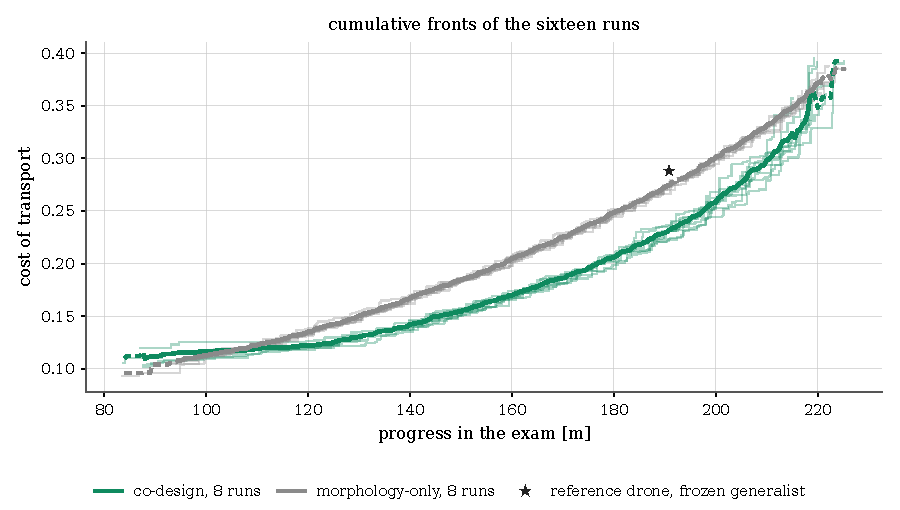
\includegraphics[width=\textwidth]{images/06_Results_and_Experiments/codesign/codesign_fronts.pdf}
\caption[The cumulative fronts of the sixteen runs]{The cumulative fronts of the sixteen runs on the exam course, co-design in green and morphology-only in grey. Thin lines are the fronts of the single runs; the thick line of each condition is, at every progress, the mean over its runs of the cost of transport of the cheapest body that reaches that progress, drawn solid where at least four of the eight fronts reach it and dashed where fewer do. The star is the reference drone flown by the frozen generalist.}
\label{fig:codesign-fronts}
\end{figure}

\autoref{fig:codesign-fronts} shows the sixteen cumulative fronts and, for each condition, the mean cost of transport at every progress over the runs whose front reaches it. The two families agree at their ends. At the tip, the farthest body of a run averages 213 to 225~m over its exam flights in the co-design runs and 217 to 226~m in the control (p-value 0.44). No body of either condition gets, on average, past 226~m of the 300~m course, so the tip is common to both conditions and is not where they differ. At the cheap end, the arm of bodies that fly 85 to 110~m for a cost of transport of 0.10 to 0.12 is the same in both conditions, and three co-design runs have no body below 128~m. Between the two ends the fronts separate, and the separation is the result of this section. From 128 to 213~m of progress the co-design fronts are cheaper at every level, with an adjusted p-value below 0.05 along the whole band. At 130, 150, 170, 190 and 210~m every one of the eight co-design runs is cheaper than every one of the eight control runs (\autoref{fig:codesign-indicators}(a), \autoref{tab:codesign-indicators}). The gap is about a sixth of the cost. At 150, 170 and 190~m the shift is $-0.031$, $-0.039$ and $-0.044$, that is 17, 17 and 16\,\% of what the control's bodies spend at those distances. The gap narrows to 12\,\% at 130~m, where the fronts begin to merge into the common arm, and to 10\,\% at 210~m, near the common tip. Read the other way, in \autoref{fig:codesign-indicators}(b), a body within a cost of transport of 0.15, 0.20 or 0.25 flies 16, 18 and 16~m farther on a co-design front than on a control front, 12, 11 and 9\,\% more. At 0.30 the gain is 10~m. At 0.35, where both fronts have reached their tips, it is 1.5~m and not significant.
% PROVENANCE: pareto_stats/summary.json (indicators, attainment band 128-213 m, progress band CoT 0.1475-0.335), indicators_per_run.csv.

\begin{figure}[htbp]
\centering
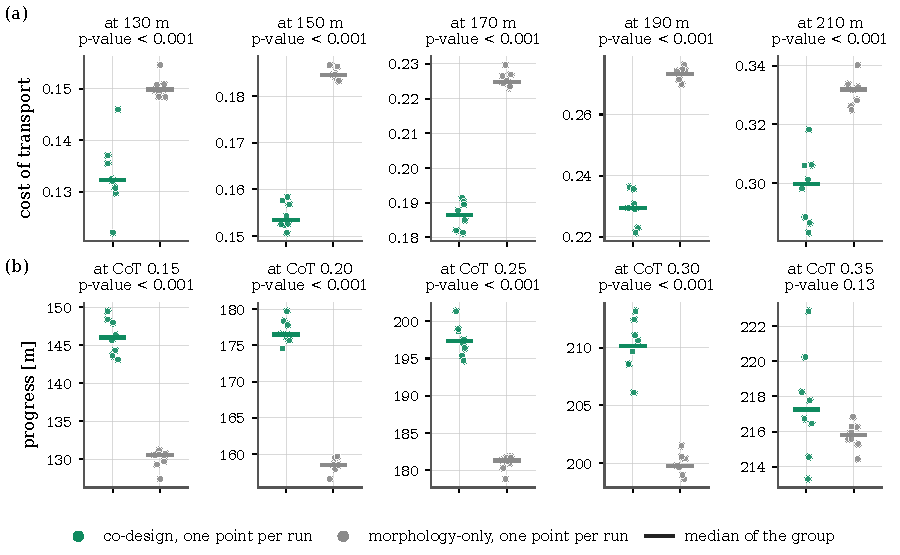
\includegraphics[width=\textwidth]{images/06_Results_and_Experiments/codesign/codesign_indicators.pdf}
\caption[The fronts read at fixed progress and at fixed cost of transport]{The fronts read at fixed progress and at fixed cost of transport, one point per run and the median of each group as a bar. (a) Cost of transport of the cheapest body of the front that reaches 130, 150, 170, 190 and 210~m. (b) Progress of the farthest body of the front within a cost of transport of 0.15, 0.20, 0.25, 0.30 and 0.35. The p-values are those of the exact rank-sum test over the sixteen runs.}
\label{fig:codesign-indicators}
\end{figure}

\begin{table}[htbp]
\centering
\small
\begin{tabularx}{\textwidth}{>{\raggedright\arraybackslash}X r r r r r}
\hline
Indicator & Co-design & Morphology-only & Shift & 95\,\% CI & p-value \\
\hline
CoT at 150~m & 0.153 & 0.185 & $-0.031$ & $-0.033$ to $-0.027$ & $< 0.001$ \\
CoT at 170~m & 0.186 & 0.225 & $-0.039$ & $-0.043$ to $-0.035$ & $< 0.001$ \\
CoT at 190~m & 0.229 & 0.273 & $-0.044$ & $-0.049$ to $-0.039$ & $< 0.001$ \\
Progress at CoT 0.15 & 146.0 & 130.5 & $+15.9$ & $+13.7$ to $+18.3$ & $< 0.001$ \\
Progress at CoT 0.20 & 176.5 & 158.5 & $+18.1$ & $+17.0$ to $+19.9$ & $< 0.001$ \\
Progress at CoT 0.25 & 197.3 & 181.3 & $+16.2$ & $+14.5$ to $+18.2$ & $< 0.001$ \\
Progress of the tip & 219.5 & 220.6 & $-1.4$ & $-5.4$ to $+2.9$ & 0.44 \\
Hypervolume & 44.8 & 41.9 & $+2.7$ & $+2.0$ to $+3.3$ & $< 0.001$ \\
\hline
\end{tabularx}
\caption[Indicators of the cumulative fronts, eight runs against eight]{Indicators of the cumulative fronts, eight runs against eight: the median over the runs of each condition, the Hodges--Lehmann shift of co-design against morphology-only with its exact 95\,\% confidence interval, and the p-value of the exact rank-sum test; the single runs are shown in \autoref{fig:codesign-indicators} and \autoref{fig:codesign-hv}. CoT is the cost of transport of the cheapest body of the front that reaches the given progress; progress, in metres, is that of the farthest body within the given cost of transport; the hypervolume is measured from the reference point at 80~m and a cost of transport of 0.5.}
\label{tab:codesign-indicators}
\end{table}

Against the reference drone, both searches find bodies that fly farther for less, but not by the same margin. The reference drone, a body of ordinary proportions flown by the generalist, lies on the mean front of the search under that generalist. The control improves on it along the front, in range and in economy at short distances, but hardly at the reference drone's own operating point. There, the cheapest body of a control run costs 0.270 to 0.276 against the reference drone's 0.288, that is 4 to 6\,\% less. The cheapest co-design body at the same 191~m costs 0.221 to 0.236, 18 to 23\,\% less.
% PROVENANCE: batch_5 brief (memory project_batch5_replication): star 190.8 m / 0.288 in all 16 runs; CoT@190 per run in indicators_per_run.csv.

\begin{figure}[htbp]
\centering
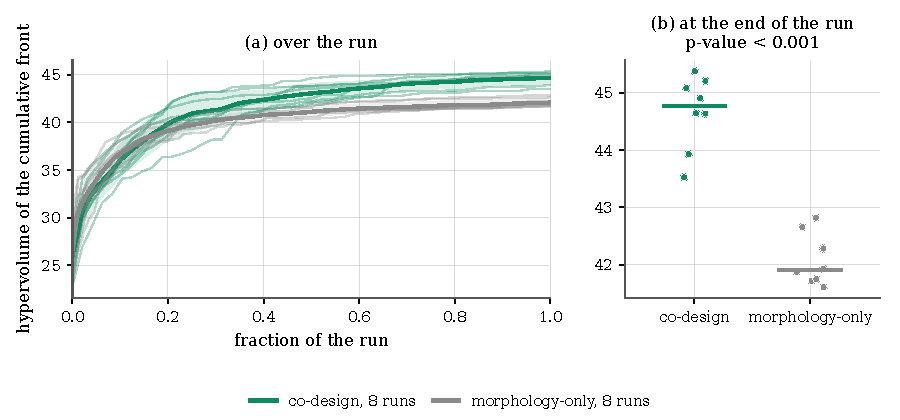
\includegraphics[width=\textwidth]{images/06_Results_and_Experiments/codesign/codesign_hv.pdf}
\caption[Hypervolume of the cumulative fronts]{Hypervolume of the cumulative fronts, reference point at 80~m and a cost of transport of 0.5. (a) Over the course of the runs, on the axis of the fraction of the run that is completed, since a co-design run holds 49 or 33 exams and a control run 87: thin lines are the single runs, thick lines the mean of each condition with a band of one standard deviation. (b) At the end of the runs, one point per run.}
\label{fig:codesign-hv}
\end{figure}

The hypervolume tells the same story in one number and adds its time course (\autoref{fig:codesign-hv}). At the end of the runs it is 43.5 to 45.4 in the co-design runs and 41.6 to 42.8 in the control, with medians of 44.8 and 41.9. The shift is $+2.7$, with a confidence interval of $[2.0, 3.3]$ and no overlap between the groups. Over the run the two curves start from the same value, since the first population is the same. The control leads for the first sixth of the run, because its bodies are updated at every generation and its first exams come faster. The co-design curve overtakes it at about a fifth of the run. The difference between the group means is significant from 36\,\% of the run to the end, after adjustment for the number of points at which it is read. The control was given more of everything that concerns the bodies, 87 exams against 49 and 5\,568 examined bodies against 3\,136, and it does not catch up.
% PROVENANCE: pareto_stats/hv_time_test.csv (cumulative HV significant from 36 % of the run), summary.json "hypervolume", exam_hv_runs_fraction_aggregate.csv.

In the terms of \autoref{ch:challenges} the comparison is as clean as the pipeline allows. The two conditions start from the same bodies, use the same operators, the same exam course and the same gate, and the control is given the larger budget. The only difference is that in one condition the 896 coefficients are searched and in the other they are held at zero. The fronts differ where there was room for them to differ, between the arm that the gate cuts and the tip that the two conditions share. They differ by up to 17\,\% of the energy per metre at equal progress and by up to 12\,\% of the progress at equal energy. \emph{This answers the question with which \autoref{sec:challenge-feasibility} closed: an adaptation that costs no more than the flights that score a body is enough to change the outcome of the search.} What it does not say is whether the outcome is a different set of bodies, or the same bodies flown better by the rules they were selected with. The next three subsections take the question apart.

\subsection{Swapping the Pareto Fronts}
\label{subsec:results-swapped-fronts}

A front of the co-design pipeline is a front of pairs: bodies selected under the rules of the moment, and rules selected on those bodies. To separate the two, the bodies of a front are flown again under a controller they were not selected with. The last front of four co-design runs and of four morphology-only runs, 37 to 44 bodies each, was rebuilt from the genomes and flown on the exam course over 256 new forests. Two controllers flew every body on the same forests: the frozen generalist, and the Hebbian controller with the best set of rules of a co-design run. The best set is the one with the highest fitness over the whole run. On a co-design front these are rules of the run in which its bodies were selected. The control runs have no rules of their own, so the bodies of their fronts were flown with the best set of rules of one of the co-design runs, the second of the four, transplanted as they were. Of the four sets of rules, that one helps the reference drone most when transplanted to it on the exam course: by 9~m over the same 256 forests, against 1 to 2~m for the other three. The choice therefore does not favour the conclusion that follows. \autoref{fig:swapped-fronts} shows one front of each kind and \autoref{tab:swapped-fronts} the eight.
% PROVENANCE: <run>/comparisons_hebbian/README.md of outer_exam_4_64_64_300_r{0,1}, outer_exam_6_64_64_300_r{0,1}, outer_morphology_only_exam_r{0..3}
% (WP2_Outer_Loop.transfer_eval, 2026-08-21, 256 forests with --forest-seed 0, exam course; the transplanted rules are exam_4_r1's best genome).
% "Best set" = best_individual/fitness/genome.npy, the all-time best by search fitness (evolve_cma.py::_finalize): generation 114 (exam_4_r0),
% 35 (exam_4_r1), 77 (exam_6_r0), 26 (exam_6_r1). Reference drone, exam course: standard_hebbian.csv 188.0 m against standard_generalist.csv 179.3 m.
% Standard drone under the four runs' rules: 180.1 / 188.0 / 179.9 / 180.9 m against 179.3 m frozen (standard_hebbian.csv).

\begin{figure}[htbp]
\centering
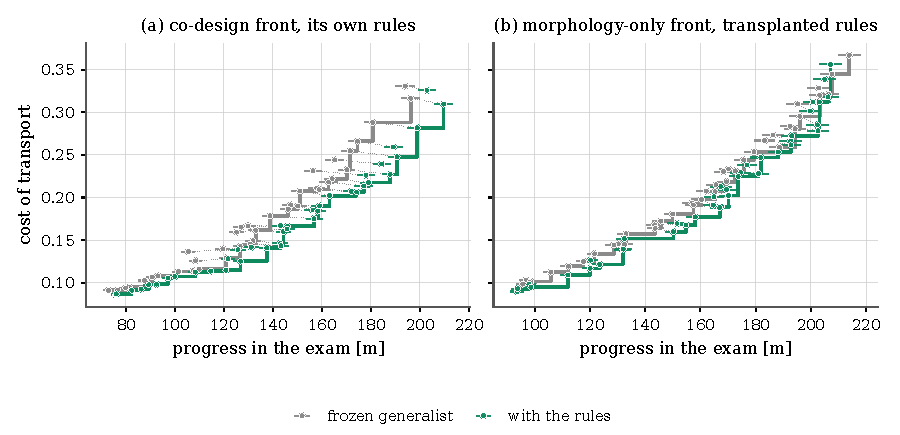
\includegraphics[width=\textwidth]{images/06_Results_and_Experiments/codesign/swapped_fronts.pdf}
\caption[Front bodies flown by the frozen generalist and by the Hebbian controller]{The bodies of a last front flown again on the exam course, over the same 256 forests, by the frozen generalist (grey) and by the Hebbian controller with the best set of rules of a co-design run (green); each body is one point in both colours, joined by a dotted line, with the standard error of its progress as a bar, and the steps are the fronts of the two sets of points. (a) A co-design front under its own rules. (b) A morphology-only front under the same rules, transplanted.}
\label{fig:swapped-fronts}
\end{figure}

\begin{table}[htbp]
\centering
\small
\begin{tabularx}{\textwidth}{>{\raggedright\arraybackslash}X r r r r r}
\hline
Front & Bodies & Rules & Progress [m] & Bodies farther & CoT \\
\hline
co-design, first run & 37 & its own & $+19.3 \pm 1.7$ & 33 & $+0.001 \pm 0.001$ \\
co-design, second run & 39 & its own & $+11.7 \pm 0.9$ & 38 & $-0.003 \pm 0.000$ \\
co-design, third run & 42 & its own & $+11.8 \pm 0.8$ & 41 & $-0.008 \pm 0.001$ \\
co-design, fourth run & 43 & its own & $+8.8 \pm 0.7$ & 43 & $-0.004 \pm 0.000$ \\
morphology-only, first run & 40 & transplanted & $+3.2 \pm 0.7$ & 28 & $-0.006 \pm 0.000$ \\
morphology-only, second run & 44 & transplanted & $+6.3 \pm 0.7$ & 38 & $-0.005 \pm 0.000$ \\
morphology-only, third run & 44 & transplanted & $+1.1 \pm 1.1$ & 25 & $-0.006 \pm 0.000$ \\
morphology-only, fourth run & 43 & transplanted & $+3.1 \pm 0.8$ & 30 & $-0.006 \pm 0.000$ \\
\hline
\end{tabularx}
\caption[What the rules add to the bodies of a front]{What the rules add to the bodies of a front: change of the mean progress and of the cost of transport of the front's bodies when they are flown by the Hebbian controller instead of the frozen generalist, on the same 256 forests of the exam course, with the standard error of the mean over the bodies, and the number of bodies that fly farther under the rules. The co-design fronts are flown with the rules of their own run, the morphology-only fronts with the rules of the second co-design run.}
\label{tab:swapped-fronts}
\end{table}

On the bodies they were selected with, the rules add 9 to 19~m of progress, and all but a handful of the bodies of every front fly farther. The front of a co-design run under its own rules lies to the right of the same bodies under the frozen generalist along its whole length (\autoref{fig:swapped-fronts}(a)). On the bodies of a morphology-only front the same rules add 1 to 6~m, three to four times less, and on one front they add nothing that the 256 forests can resolve; the two fronts of panel (b) nearly coincide in progress. What transfers is the economy. The cost of transport falls by 0.005 to 0.006 on every front of the control, on almost every body, as it falls on three of the four co-design fronts. This is the saving that \autoref{sec:inner-loop-experiments} found the rules give to any base controller on a fixed body. The progress does not transfer. The rules let a co-design front fly farther than the generalist would fly it, but only on the bodies they were evolved with, and not on bodies that were selected under the generalist. \emph{A co-design front is therefore not the front of the generalist with a better controller on top.} The rules have specialized to the family of bodies that the outer loop retained, and the bodies were retained because the rules fly them, so what the front holds is the pair. This is the reversal of \eqref{eq:ranking-flip} seen from its far side: a body selected under an adapting controller is one whose value shows with a controller adapted to it.

\subsection{PCA Analysis of the Evolved Morphologies}
\label{subsec:results-pca}

If the co-design front holds pairs, the bodies of the two conditions can be compared directly, in the space of the genome. Do the two searches, started from the same 64 bodies, go to the same place? The population of a run at each phase is summarized by its centroid in the unit cube of the 15 genes of \autoref{tab:drone-genome}, and a run by the path of that centroid from the first phase to the last. Distances between centroids are taken in the 15 dimensions of the cube. There, a distance of 0.7 corresponds to a difference of about 0.18 on every gene, or 18\,\% of its range. The principal components serve the figure only. For each of the six seeds a PCA is fitted on the centroids of its two runs, and the first two components carry 50 to 58\,\% of their variance (\autoref{fig:pca-seed-pairs}).
% PROVENANCE: WP2_Outer_Loop.pca_trajectories --per-seed (logs/remote/outer_nsga/pca_exam_seed_pairs_independent/, seed_pair_distances.csv,
% seed_pair_pca_variance.csv); joint 14-run distances in pca_exam_seed_paired/final_centroid_distances.csv (refresh-6 runs included there).

\begin{figure}[htbp]
\centering
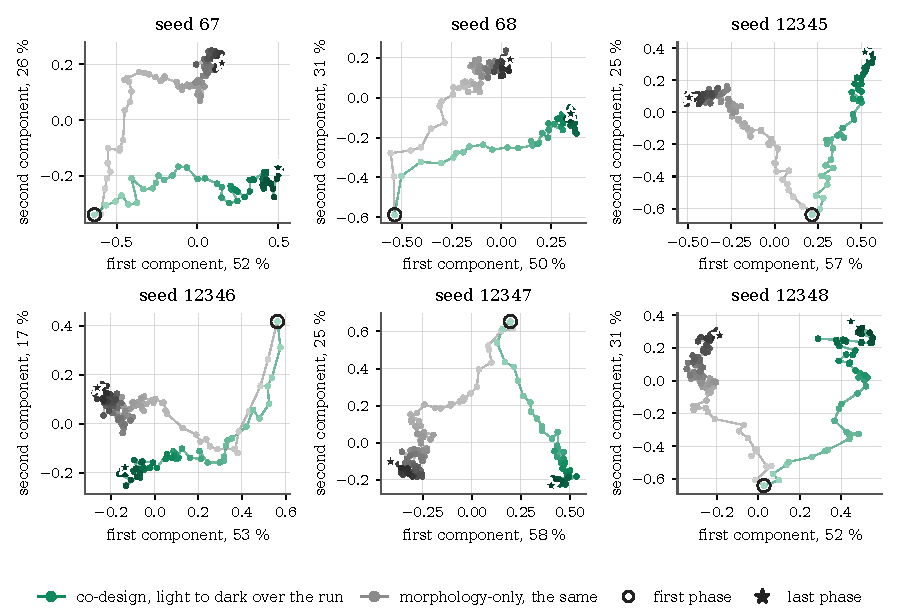
\includegraphics[width=\textwidth]{images/06_Results_and_Experiments/codesign/pca_seed_pairs.pdf}
\caption[The path of the population of the two runs of each seed in the space of the genome]{The path of the population of the two runs of each seed in the space of the genome, one panel per seed: the centroid of the 64 bodies at every phase, from the first (circle) to the last (star), co-design in green and morphology-only in grey, darker as the run proceeds. Each panel has its own principal components, fitted on the centroids of its two runs, with the share of the variance each carries on its axis; the axes are not comparable across panels.}
\label{fig:pca-seed-pairs}
\end{figure}

\begin{table}[htbp]
\centering
\begin{tabularx}{\textwidth}{>{\raggedright\arraybackslash}X r r r}
\hline
Pair of runs & Pairs & Distance & Range \\
\hline
two morphology-only runs & 28 & $0.57 \pm 0.17$ & 0.28 to 0.94 \\
two co-design runs & 28 & $0.70 \pm 0.15$ & 0.38 to 0.99 \\
a co-design and a morphology-only run, same seed & 8 & $0.70 \pm 0.20$ & 0.50 to 1.08 \\
a co-design and a morphology-only run, different seeds & 56 & $0.74 \pm 0.13$ & 0.48 to 1.04 \\
\hline
\end{tabularx}
\caption[Distances between the last populations of the runs]{Distances between the centroids of the last populations of the sixteen runs, in the unit cube of the genome, by kind of pair: mean, standard deviation and range over the pairs. The two co-design runs with phases of six generations are included; the paired distances of the six seeds of \autoref{fig:pca-seed-pairs} are 0.59, 0.50, 1.08, 0.51, 0.90 and 0.69.}
\label{tab:pca-distances}
\end{table}

In every panel of \autoref{fig:pca-seed-pairs} the two runs leave the same point together and part within the first five phases. Each run moves about 1.0 in the unit cube from the common starting point. Three of the six pairs end 0.69, 0.90 and 1.08 apart, farther than any two of the seven clustered control runs. The other three end 0.50 to 0.59 apart, which is the distance between two control runs of different seeds (\autoref{tab:pca-distances}). Two things follow from the table. First, the starting bodies do not decide where a run ends. A co-design run is no closer to the control run that started from its own 64 bodies than to a control run that started from others, 0.70 against 0.74. For only one of the eight co-design runs is its seed partner the nearest control run. Second, the two conditions do not scatter alike. Seven of the eight morphology-only runs end within 0.28 to 0.62 of each other, in one cluster. The eighth, one of the two runs without a co-design partner, ends 0.72 to 0.94 from the other seven. Under a fixed controller the search over bodies thus has one main optimum, which seven runs find, and at least one other. The co-design runs end 0.38 to 0.99 apart, 0.70 on average against 0.49 for the seven. They also end farther from the cluster: the control run nearest to a co-design run is 0.48 to 0.75 away, where the control run nearest to one of the seven is 0.28 to 0.48 away. \emph{The adapting controller does not shift the optimum of the body search by a fixed amount: it changes which bodies come first, as \autoref{sec:challenge-morphology} argued it would, and the bodies it makes reachable are different ones for different runs.} Which bodies these are, in terms a designer can read, is the subject of the next subsection.
% PROVENANCE: tesis/scripts/pca_distances_16runs.py -> images/06_Results_and_Experiments/codesign/pca_distances_16runs.json (2026-10-01, all sixteen
% runs; the earlier table used final_centroid_distances.csv, which lacks the control runs of seeds 69 and 70). Seven clustered controls 0.487 +- 0.094
% (0.278-0.618); seed 70 to the seven 0.718-0.945; nearest control of a co-design run 0.476-0.746; nearest fellow among the seven 0.278-0.475;
% seed partner nearest for 1 of 8 (cod6_s68). Seed pairs 67/68/12345/12346/12347/12348: final distance 0.59/0.50/1.08/0.51/0.90/0.69, moves 0.93-1.20,
% cosine of the two moves 0.87/0.89/0.52/0.85/0.58/0.80. Author's decision 2026-10-01: count by distance (three of six), not by panel (five of six).

\subsection{Morphology Choices of The Evolution}
\label{subsec:results-morphologies}

\begin{figure}[htbp]
\centering
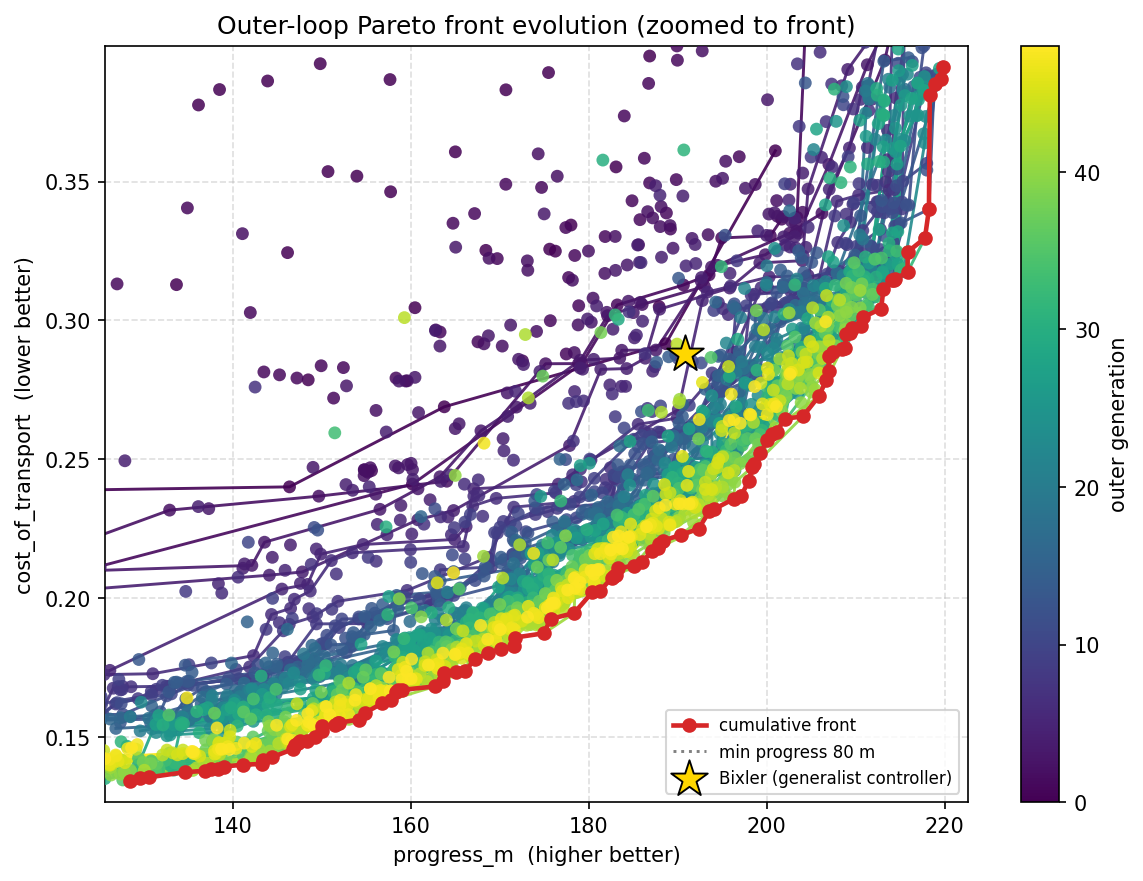
\includegraphics[width=0.8\textwidth]{images/06_Results_and_Experiments/front_evolution/exam4_r0_pareto_front_evolution_zoomed.png}
\caption[The examined bodies of a co-design run]{The examined bodies of the first co-design run in the plane of the objectives, coloured by the phase of their exam, with the cumulative front of the run in red; bodies below 128~m of progress are left out of the view. The lines join the successive exams of the bodies that survived more than one phase.}
\label{fig:front-evolution}
\end{figure}

\autoref{fig:front-evolution} shows what a run does with its bodies: the 3\,136 examined bodies of the first co-design run, coloured by phase. The early exams scatter above the front and the later ones lie along it. The front itself is built over the whole run: its cheap end comes from bodies of the middle phases and its tip from a body of the thirteenth phase. The two ends of a front are two designs, and \autoref{fig:champions} shows the two of this run: the body that flies farthest, 220~m at a cost of transport of 0.39, and the cheapest body that passes the gate, 128~m at 0.13. \autoref{tab:champions} gives their parameters.
% PROVENANCE: outer_exam_4_64_64_300_r0/2026-08-10_21-53-50_.../plots/champion_renders/champions.csv (progress champion phase 13, CoT champion
% phase 35, gated at 80 m), URDF masses parsed from the champion URDFs (0.575 and 1.963 kg, wing links 0.152 and 1.453 kg).

\begin{figure}[htbp]
\centering
\begin{subfigure}[c]{0.48\textwidth}
\centering
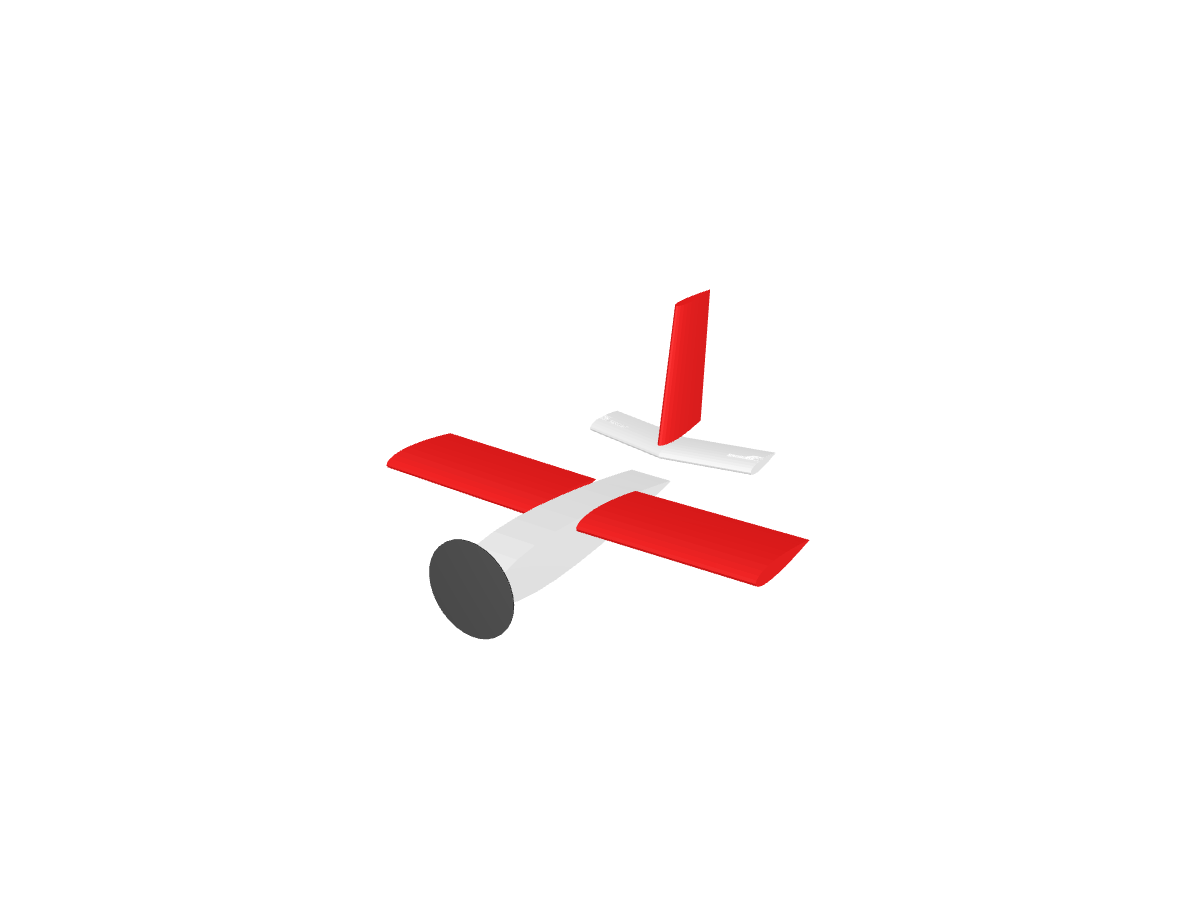
\includegraphics[width=\textwidth, trim={60 100 60 100}, clip]{images/06_Results_and_Experiments/champion_renders/outer_exam_4_64_64_300_r0/progress_champion_gen13_ind_001_3quarter.png}
\caption{}
\label{fig:champions-progress-3q}
\end{subfigure}
\hfill
\begin{subfigure}[c]{0.48\textwidth}
\centering
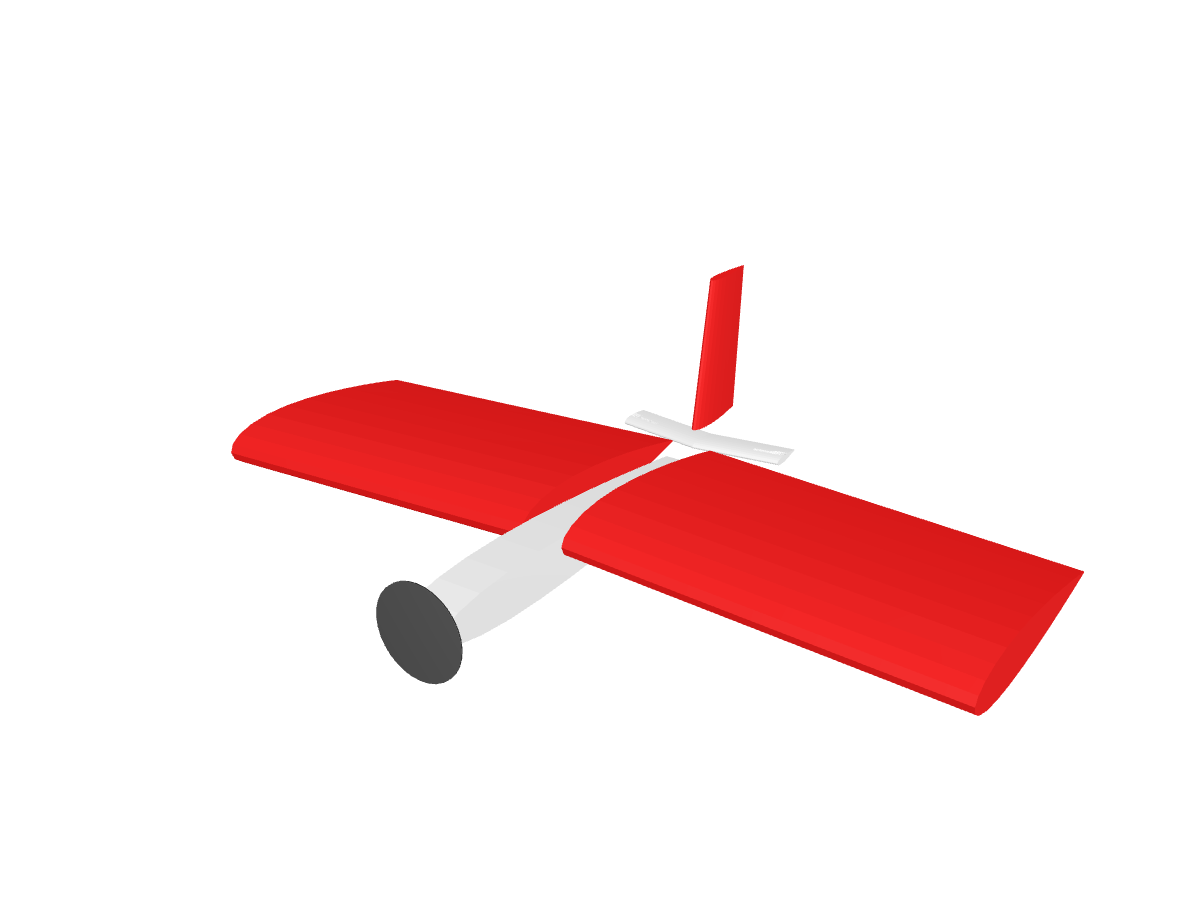
\includegraphics[width=\textwidth, trim={60 100 60 100}, clip]{images/06_Results_and_Experiments/champion_renders/outer_exam_4_64_64_300_r0/cot_champion_gated80m_gen35_ind_000_3quarter.png}
\caption{}
\label{fig:champions-cot-3q}
\end{subfigure}
\begin{subfigure}[c]{0.48\textwidth}
\centering

\includegraphics[width=\textwidth, trim={60 100 60 100}, clip]{images/06_Results_and_Experiments/champion_renders/outer_exam_4_64_64_300_r0/progress_champion_gen13_ind_001_top.png}
\caption{}
\label{fig:champions-progress-top}
\end{subfigure}
\hfill
\begin{subfigure}[c]{0.48\textwidth}
\centering

\includegraphics[width=\textwidth, trim={60 100 60 100}, clip]{images/06_Results_and_Experiments/champion_renders/outer_exam_4_64_64_300_r0/cot_champion_gated80m_gen35_ind_000_top.png}
\caption{}
\label{fig:champions-cot-top}
\end{subfigure}
\caption[The two ends of the front of a co-design run]{The two ends of the front of the first co-design run, drawn at one common scale. Left, (a) and (c): the body that flies farthest. Right, (b) and (d): the cheapest body that passes the gate. Three-quarter views above, top views with the nose up below; wing panels and rudder in red, fuselage and elevator in grey.}
\label{fig:champions}
\end{figure}

\begin{table}[htbp]
\centering
\begin{tabularx}{\textwidth}{>{\raggedright\arraybackslash}X r r}
\hline
 & Farthest body & Cheapest body \\
\hline
Progress and cost of transport in the exam & 220~m, 0.39 & 128~m, 0.13 \\
Span of one wing panel & 0.40~m & 0.85~m \\
Chord of the wing & 0.21~m & 0.56~m \\
Wing area, both panels & 0.17~m$^2$ & 0.95~m$^2$ \\
Length of the fuselage & 0.61~m & 0.90~m \\
Centre of mass along the fuselage & 56\,\% & 31\,\% \\
Attachment of the wing along the fuselage & 52\,\% & 56\,\% \\
Span of the elevator, of the rudder & 0.42~m, 0.33~m & 0.41~m, 0.37~m \\
Dihedral & $-0.9^{\circ}$ & $+2.8^{\circ}$ \\
Gear ratios of the sweep, of the twist & 3.19, 2.22 & 3.18, 2.21 \\
Airfoil & NACA 4417 & NACA 4520 \\
Mass, of which the wing & 0.58~kg, 0.15 & 1.96~kg, 1.45 \\
\hline
\end{tabularx}
\caption[The two bodies at the ends of the front of a co-design run]{The two bodies of \autoref{fig:champions}: the genes of \autoref{tab:drone-genome} in physical units, the wing area and the mass of the built body. The chord follows from the span and the aspect ratio of the panel.}
\label{tab:champions}
\end{table}

The two bodies are as different as the design space allows on its main axes, and alike on the others. The body that flies farthest is small and light. It has panels of 0.40~m, a wing of 0.17~m$^2$, a fuselage of 0.61~m and a mass of 0.58~kg in all. Its centre of mass is well aft, at 56\,\% of the fuselage, close to the wing. It is a body with little static margin: its centre of mass lies close to the aerodynamic centre of the whole aircraft, so it turns readily. This is what the dense half of the course rewards, and it pays for the agility with a cost of transport three times that of the other body. The cheapest body is a glider. It has panels of 0.85~m with a chord of 0.56~m, 1.8~m from tip to tip, a wing of almost a square metre that weighs 1.45 of the body's 1.96~kg, a long fuselage with the centre of mass forward, at 31\,\%, and a positive dihedral. All of this makes for a stable and slow flight. It does not get through the second half of the course, where the forest thickens past what such a wing can be steered through: it stops at 128~m on average, four metres from the point where the front meets the common arm. The two bodies agree on their gear ratios, 3.2 for the sweep and 2.2 for the twist, near the top of the range for the sweep, and on a cambered airfoil. A run that reaches both ends of the front from one population reaches them with the same actuation, inherited along the way, and moves the wing and the fuselage instead.

\begin{figure}[htbp]
\centering
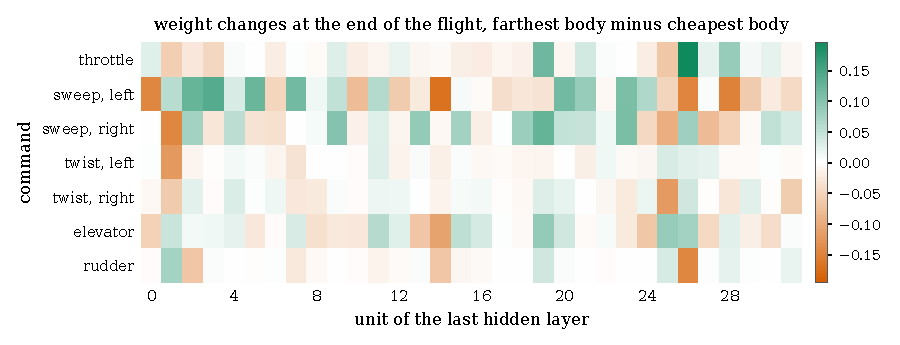
\includegraphics[width=\textwidth]{images/06_Results_and_Experiments/codesign/champion_deltaw.pdf}
\caption[Difference of the plastic weights on the two bodies]{Difference between the changes of the output weights, $\mat{W}_t - \mat{W}_0$ at the end of the flight, that the last set of rules of the run produces on the two bodies of \autoref{fig:champions}, flown on the same forest: one row per command, one column per unit of the last hidden layer, green where the farthest body's weight moved further up, orange where the cheapest body's did.}
\label{fig:champion-deltaw}
\end{figure}

The same rules do not do the same thing on the two bodies. \autoref{fig:champion-deltaw} compares the changes of the output weights at the end of a flight of each body under the best set of rules of the last generation of the run, on the same longer evaluation forest of 630~m, at a commanded speed of 12~m/s. The farthest body completes the forest in 54~s; the cheapest one flies 317~m and collides after 28~s. The two matrices of weight changes correlate at 0.76 over their 224 entries, and at 0.83 when the first is read at the same instant as the second ends. Where they differ, they differ most in the rows of the two sweep commands, by up to 0.20 where the trained weights have a mean magnitude of 0.05. This is one flight of each body and no more than an illustration. But it shows what \autoref{subsec:hebbian-why-output} asked of the plastic layer: the same rules, given a different body, arrive at different weights, and the difference is concentrated on the commands by which the two bodies differ most in what they can do.
% PROVENANCE: outer_exam_4_64_64_300_r0/.../plots/champion_videos/deltaw/deltaw_summary.csv (corr_final 0.7629, corr_matched 0.8260,
% max_abs_diff 0.1961, t 53.96 / 28.08 s, 630 m corridor seed 50, 12 m/s, controller_gen199_best_idx027).

\subsection{Generalization Capabilities of Evolved Controllers}
\label{subsec:results-generality}

The last question is what becomes of the rules. As \autoref{subsec:pipeline-run} anticipated, rules selected on bodies that resemble each other more at every update are asked to fly a family rather than anything, and \autoref{subsec:results-swapped-fronts} found that their gain in progress does not transfer to bodies of another front. Two measurements follow this along the run. The first is taken in every co-design run, at every generation, as described in \autoref{subsec:pipeline-run}. The best set of rules of the generation and the frozen generalist fly the reference drone, a body that is never in the population, on 4\,096 new forests of the search course. Over the first twenty generations the two differ by less than one point of fitness in all eight runs, in either direction. Over the last twenty generations the rules are below the frozen generalist by 10 to 16 points in all eight runs, flying 107 to 111~m of the course where the generalist flies 117~m. The loss grows monotonically along the run, and there is no early window in which the rules fly the reference drone better than the controller without rules.
% PROVENANCE: results/validation_summary.csv of the 8 co-design runs, best - baseline: first 20 gens -1.0..+0.4, last 20 gens -10.1..-16.1;
% progress last 20 gens 107.0..110.7 vs 116.7..116.8 m (computed 2026-09-29).

\begin{figure}[htbp]
\centering
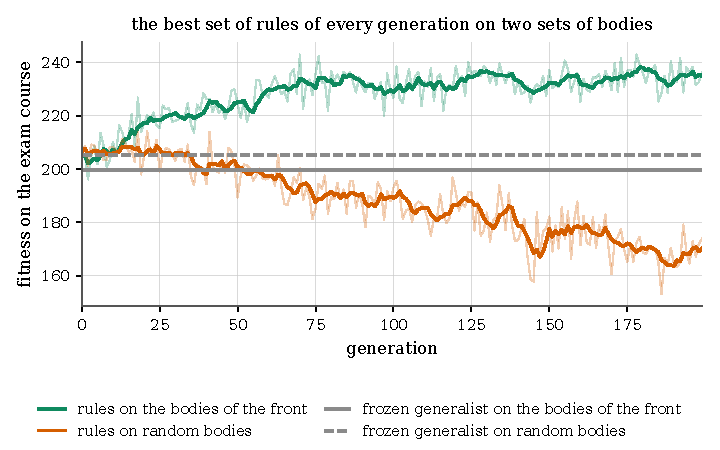
\includegraphics[width=0.8\textwidth]{images/06_Results_and_Experiments/codesign/generality_fitness.pdf}
\caption[The best set of rules of every generation on the bodies of the front and on random bodies]{The best set of rules of every generation of the first co-design run, flown on the 37 bodies of the run's last front (green) and on 128 bodies drawn at random from the design space (orange), over the same 64 forests of the exam course for every controller: fitness, mean over the bodies; thin lines are the raw values, thick lines a moving average over five generations. The grey lines are the frozen generalist on the same bodies and forests.}
\label{fig:generality}
\end{figure}

The second measurement asks the same question of the bodies the rules were selected for and of bodies they never met, on the same course as the exam (\autoref{fig:generality}). For the first co-design run, the best set of rules of each of the 200 generations was flown on the 37 bodies of the run's last front and on 128 bodies drawn at random from the design space, as the first population is. Every controller flew the same 64 forests of the exam course, next to the frozen generalist on the same bodies and forests. On the front bodies the rules of the first 25 generations already add 11 points of fitness and 8~m of progress to the frozen generalist. The gain grows to 29 points and 19~m by generations 50 to 74, and it levels off from generation 75 at 32 to 36 points and 22 to 25~m, 17\,\% of the fitness, with every one of the 37 bodies flying farther, while their cost of transport does not move. On the random bodies the same rules add 2 points in the first 25 generations, nothing that the 128 bodies can resolve, and they lose from then on without pause: 10 points by generations 50 to 74, 27 points by generations 125 to 149, and 37 points and 26~m of progress in the last 25 generations, an 18\,\% loss. Against this loss stands a saving of 0.01 to 0.02 in cost of transport, which is the portable economy of \autoref{subsec:results-swapped-fronts} once more.
% PROVENANCE: outer_exam_4_64_64_300_r0/.../generality/summary.csv (WP2_Outer_Loop.controller_generality, 2026-08-31): front n 37, random n 128,
% 64 exam forests, 201 controllers; block means recomputed 2026-09-29 (front +11.4/+29.2/+35.5, random +1.8/-10.4/-36.9 fitness).

The two curves are what specialization looks like. The gain on the bodies of the front saturates within the first half of the run, when the family of bodies has largely formed. The loss on bodies outside the front goes on to the last generation. The rules are therefore not simply degrading: they are following the bodies that the outer loop keeps, whose population narrows in the meantime from a mean pairwise distance of 1.56 in the genome cube at the first phase to 0.70 at the last. \emph{What the pipeline pays for its front is the generality of the controller it started from.} The rules that fly the evolved bodies 17\,\% better than the frozen generalist fly a random body 18\,\% worse and the reference drone 6 to 9\,\% worse. They could not be reused on another family of bodies without being evolved again, as \autoref{subsec:results-swapped-fronts} showed at the scale of a front. For the search this is not a defect. The controller was paid for once, as \autoref{sec:challenge-feasibility} required, and the adaptation of its output layer to the bodies being scored is what the rules provide at the cost of the flights. That the adaptation is to the family the search retains, rather than to every body in the space, is what makes it cheap.
% PROVENANCE: population diversity computed 2026-09-29 from outer_population.csv (first phase 1.55-1.57 in all 16 runs, last phase 0.69-0.95
% co-design, 0.75-0.92 morphology-only: the control narrows as much, so this is stated for the run of the figure only).